\chapter[CVAEs for real GW events]{Conditional variational autoencoders for detecting real GW signals}

In this chapter I will discuss some recent soon to be published work on using the \texttt{VItamin} machine learning for gravitational wave parameter estimation pipeline to do Bayesian PE on real \ac{GW} signals. In the first section I will introduce the problem, in the second I will discuss data pre-processing and generation, in the third section I will discuss results in both real and Gaussian noise cases on a variety of real \ac{GW} signals.

\section{Introduction}

\section{Signal pre-processing/generation}

\section{Training tricks}

\subsection{Data augmentation}

In addition to allowing the network to see multiple noise realizations 
of the same signal multiple times, every time we give the network 
a new chunk of signals, we also randomize the phase, time of arrival and 
distance of the new loaded in training samples.

%
% Distance augmentation
%
For distance, we first choose values uniformly at random from 0 to 1 for 
each distance training sample parameter. These values are then 
converted to units of Mpc by 

\begin{equation}\label{eq:dist_rescale}
    d_{\textrm{new}} = d_{\textrm{min}} + d_{\textrm{uni}}*(d_{\textrm{max}} - d_{\textrm{min}}),
\end{equation}

where $d_{\textrm{uni}}$ is a uniform set of numbers between 0 and 1, 
$d_{\textrm{max}}$ represents the maximum allowed distance according to the prior and $d_{\textrm{min}}$ is the minimum allowed distance according to the prior. We then determine the factor by which the distance has changed from its old value for each training sample by dividing the old distance by the new distance value.

\begin{equation}
    d_{\textrm{corr}} = \frac{d_{\textrm{old}}}{d_{\textrm{new}}}
\end{equation}

where $d_{\textrm{old}}$ is the original distance value for the sample 
and $d_{\textrm{new}}$ is the new value. 

%
% Phase augmentation
%

In order to get the phase augmentation scale term 
we do a similar process as the distance 
augmentation above. We again choose a uniform value between 0 and 1 and 
apply the same rescaling as that in equation \ref{eq:dist_rescale}, but 
instead with bounds relavent to phase (0 to $\pi$). Bounds are only 
up to a maximum of $\pi$ due an applied reparameterization trick 
discussed below in subsection \ref{subsec:phipsi_repar}. A phase 
correction term is then calculated

\begin{equation}
    \phi_{\textrm{corr}} = -1.0 \times (\cos(\phi_{\textrm{new}} - \phi_{\textrm{old}}) + \sin(\phi_{\textrm{new}} - \phi_{\textrm{old}}) \times i),
\end{equation}

where $\phi_{\textrm{corr}}$ is the phase correction factor we 
will use to randomize the phase, $\phi_{\textrm{new}}$ is the new 
randomized phase value and $\phi_{\textrm{old}}$ is the original 
training sample phase value.

%
% time correction
%

The time scale term is then computed by again choosing a random value 
between 0 and 1 for all training samples and rescaling those random 
values to be in units of seconds which are between the allowable 
prior bounds of time. We then convert the new randomized time 
to radians and find the difference between the new and old 
times

\begin{equation}
    t_{\textrm{corr}} = -2.0\pi (t_{\textrm{new}} - t_{\textrm{old}}),
\end{equation}

where $t_{\textrm{new}}$ is the new time of coalescence, $t_{\textrm{old}}$ 
is the old time of coalescence and $t_{\textrm{corr}}$ is the time of coalesence scale factor. The complex value for the time of coalesence 
scale factor $t_{\textrm{corr}}$ is computed 

\begin{equation}
    t_{\textrm{corr}} = -1.0 \times (\cos(t_{\textrm{corr}}) + \sin(t_{\textrm{corr}}) \times i).
\end{equation}

Finally, given all the correction factors for time $t_{\textrm{corr}}$, 
distance $d_{\textrm{corr}}$ and phase $\phi_{\textrm{corr}}$ have been 
calculated, we need only simply multiply 
the phase correction term and the time correction term by the real 
\ac{FFT} of the training sample time series

\begin{equation}
    y_{\phi \textrm{corr}} = \mathcal{F}(y) \times \phi_{\textrm{corr}} \times t_{\textrm{corr}},
\end{equation}

where $\mathcal{F}$ is the real \ac{FFT}. To apply the distance term 
apply the inverse real \ac{FFT} and multiply by the distance correction 
scale factor

\begin{equation}
    y_{\phi \textrm{corr}} = \mathcal{F}^{-1}(y_{\phi \textrm{corr}}) \times d_{\textrm{corr}}. 
\end{equation}

Adding these randomized elements to the existing training workflow 
was absolutely key in ensuring that the neural network model did 
not overfit the training set.

\subsection{Phase and Psi reparameterization trick}\label{subsec:phipsi_repar}

One of the single biggest issues we have faced while training the neural network 
has been dealing with the multi-modal nature of the phase ($\phi$) and psi 
($\psi$) parameters. Along with the addition of the Gaussian mixture model 
component of the network mentioned previously, we have also implemented 
a reparameterization of both phase and psi in order to simplify the 
search space for the neural network partly inspired by the work of Jones in \cite{10.1093/mnras/stv1584}.

In order to 
go from $\psi$ and $\phi$ to a new representation $\psi$ and $X$, we first take the 
remainder of $\psi + \phi$ divided by $\pi$ which then becomes a new parameter denoted as $X$.
We also take the remainder of $\psi$ divided by $\frac{\pi}{2}$.

\begin{equation}
    X = (\psi + \phi) \textrm{ mod } \pi.
\end{equation}
\begin{equation}
    \psi = \psi \textrm{ mod } \frac{\pi}{2}. 
\end{equation}

In order to get back to the original $\psi, \phi$ representation, we choose a set of two random integers between zero 
and $2$ ($D_1$) multiplied by $\pi$, as well as a set of two random integers between $0$ and $\frac{1}{2}$ ($D_2$)
multiplied by $\pi$ for each $\psi$ value and ensure both $\psi$ and $X$ are in radians.

\begin{equation}
    D_{1}=\left\{ x\in\mathbb{Z}|0\leq x\leq 2 \right\} \times \pi
\end{equation}

\begin{equation}
    D_{2}=\left\{ x\in\mathbb{Z}|0\leq x\leq \frac{1}{2} \right\} \times \pi
\end{equation}

We then subtract off $\psi$ from $X$, add both random radian integers and take the modulus 
of the whole expression with respect to $2\pi$ in order to get back $\phi$. 

\begin{equation}
    \phi = ((X - \psi) + D_{1} + D_{2}) \textrm{ mod } 2\pi     
\end{equation}

For $\psi$ we add set $D_2$ and take the modulus with respect to $\pi$

\begin{equation}
    \psi = (\psi + D_2) \textrm{ mod } \pi.
\end{equation}

This essentially tessellates the $X-\psi$ and $\psi$ parameters across 
four quadrants of the parameter space while maintaining the same number of samples and 
 general distribution shape.

The reparameterization process is visually illustrated in Figure \ref{fig:Xpsi}. It can be clearly seen 
that the 2D representation $X, \psi$ in both the upper left and lower right subplots, is vastly 
simpler than the original 2D $\phi, \psi$ representation. The transformation also 
is able to maintain the property of being fully-reversible. Although, we do note that 
if one considers \ac{GW} template waveforms with higher order modes this degeneracy is 
broken and the above reparameterization would not be necessary \cite{10.1093/mnras/stv1584}.

\begin{figure}
    \centering
    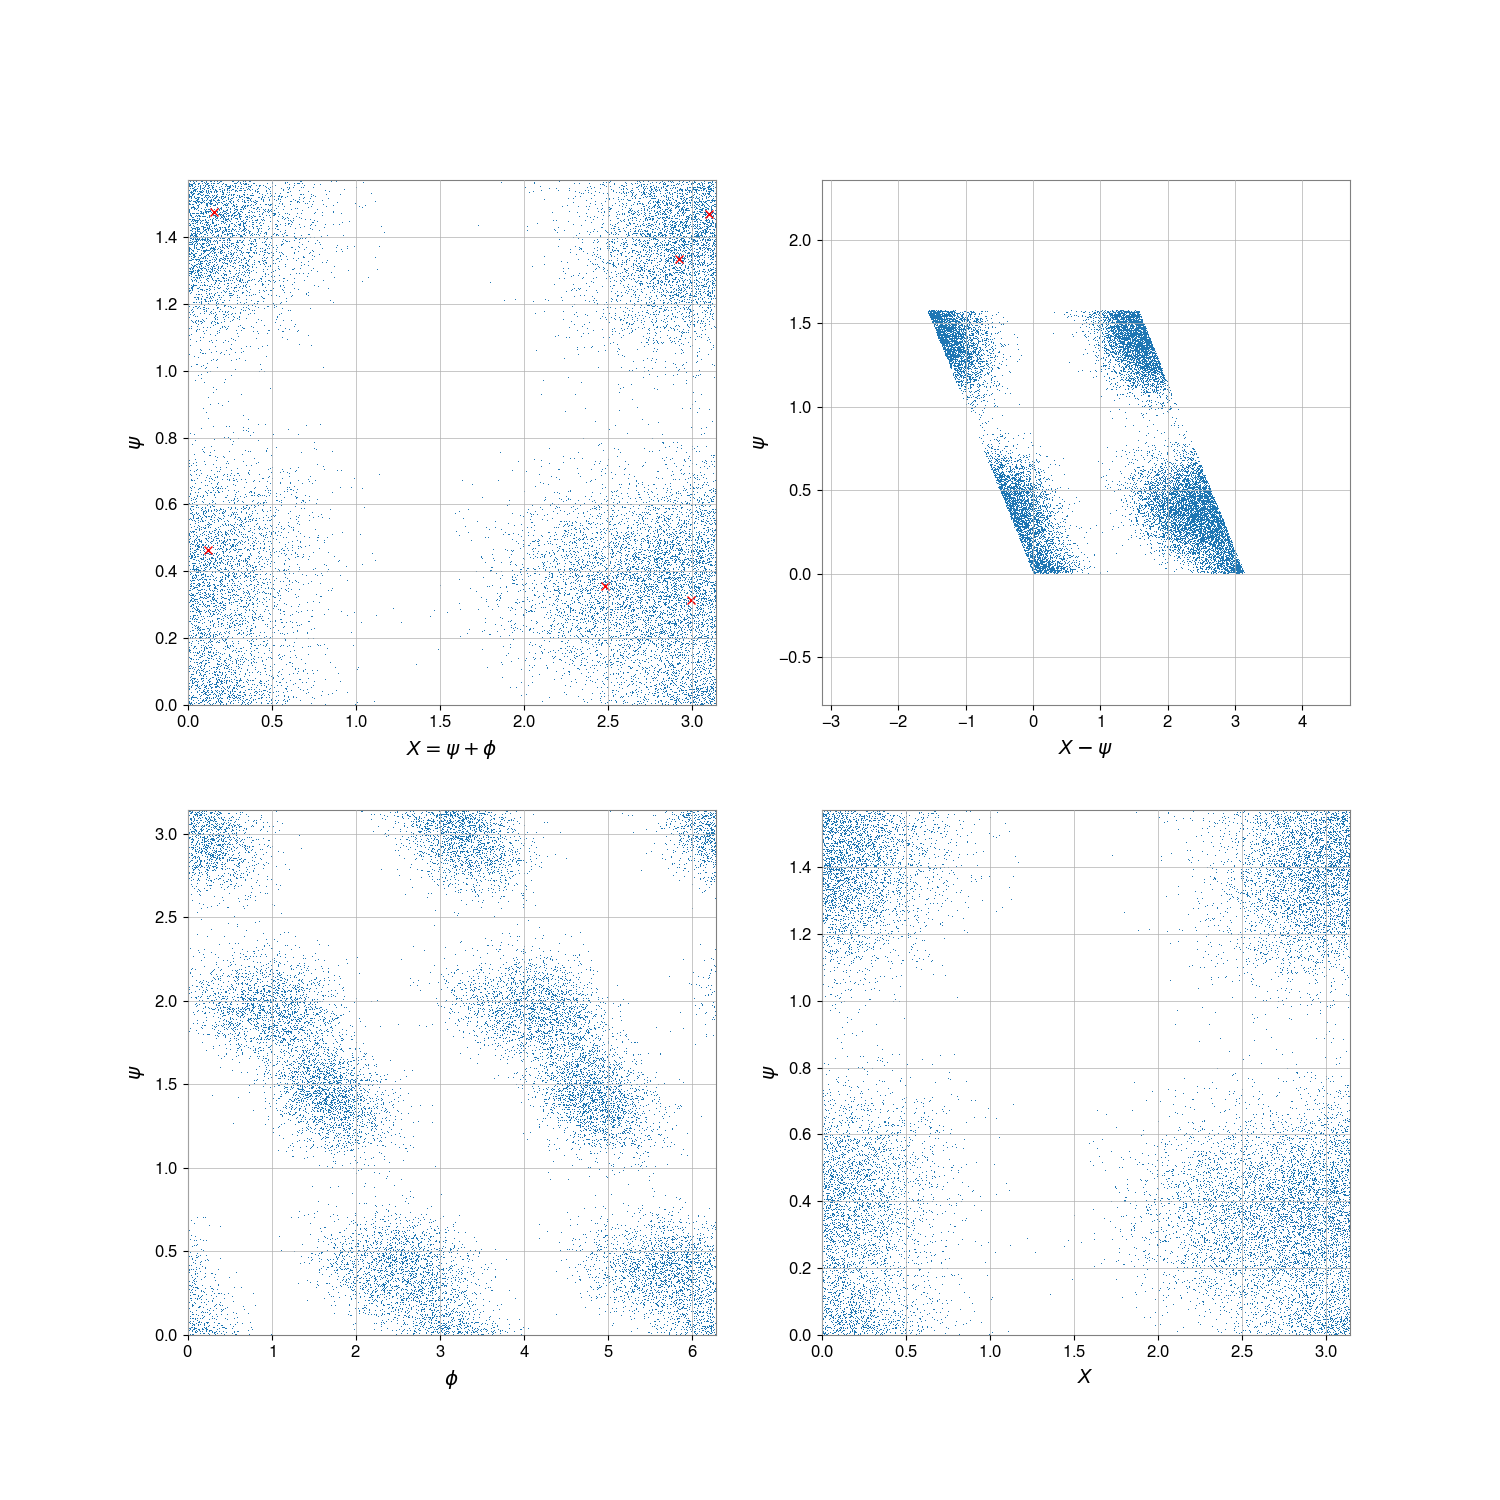
\includegraphics[width=16cm,height=20cm,keepaspectratio]{figures/Xpsi.png}
    \caption[An illustration of the $\psi$ and $\phi$ reparameterization trick.]{An illustration of the $\psi$ and $\phi$ reparameterization trick. Upper left 
    plot: a random set of samples drawn from randomly generated multivariate Gaussian distributions for both $\psi$ and $\phi$. Red cross hairs denote Each Gaussian's mean and $X$ represents a reparameterization of $\psi$ and $\phi$. Upper right: Same plot as the upper right, but with $\psi$ subtracted off from the reparameterization in 
    order to form a trapezoidal-like shape for tessellation purposes. Lower left: We then apply a tessellation of the samples in the upper right figure in order to convert the reparameterization back to the original units of $\psi$ and $\phi$. Lower right: We can get back to the reparameterized version by applying our reparameterization trick again without any change to the original in the upper left.}
    \label{fig:Xpsi}
\end{figure}



\section{Results}

\section{Conclusions}

